

\section{Intro to \LaTeX{} (\& \texttt{reledmac})}

\begin{frame}{Producing PDFs\dots}
    \metroset{block=fill}
    Why are we doing this workshop? The motivation from our abstract:
    \begin{itemize}
        \item[\textcolor{w3schools}{\faCheck}] But what happens after an edition is encoded in TEI? 
        \item[\textcolor{w3schools}{\faHandORight}] While it is an \textbf{ideal format for archiving digital data}, it is \alert{less than ideal for viewing and interacting with the edited text.}
        \item[\textcolor{w3schools}{\faHandORight}] The data transformation language XSLT allows editors to create multiple representations from their data encoded in XML, enabling the creation of both digital and print editions. 
    \end{itemize}
    
    \begin{block}{Goals for the next session}
    \begin{enumerate}
        \item[\textcolor{w3schools}{\faCheck}] learn some theory basics
        \item[\textcolor{w3schools}{\faCheck}] everybody on the same page on XML/TEI for digital editing
        \item[\textcolor{w3schools}{\faCheck}] creating websites in HTML (\& Bootstrap)
        \item[\textcolor{alert}{\faClose}] creating PDFs \& print(able) editions using \LaTeX{} (\& \texttt{reledmac})
    \end{enumerate}
    \end{block}
\end{frame}

%-----------------------------------------------------

%-------------------------------
\begin{frame}[fragile]{\LaTeX{}}

\begin{columns}
\column{0.55\textwidth}\small 
\begin{itemize}
    \item \bg{w3schools}{white}{.tex} Typesetting with \TeX{} using Lamport macros (i.e. shortcuts to make complicated code easy)
\item \LaTeX{} reads in those macros (with telling names like \verb|\emph{}| for `emphasis', an `intelligent' command which can be redefined for the whole document)
\item feels like markup for those producing the code (illusion of descriptive markup)
\item placeholder for complex procedural language 
\item \textbf{WYIWYG}-Editors (\emph{what you see is what you get}, i.e. MS Word) vs. \textbf{WYSIWYM} (\emph{what you see is what you mean} $\to$ \LaTeX{}) 
\end{itemize}
\column{0.45\textwidth}
\footnotesize
\metroset{block=fill}
\begin{block}{Example commands}
Commands below without the spaces \\
\mycommand{\textit{Italic}}{\textit{Italic} (presentational.)}
\mycommand{\emph{Italic}}{\textit{Italic} (semantic/`intelligent')}
\mycommand{\textbf{Bold}}{\textbf{bold face}}
\mycommand{\section{Title}}{Heading 1}
\mycommand{\subsection{Subtitle}}{etc.}
\mycommand{\href{http://a.com}{Link}}{\href{https://www.latex-project.org/latex3/}{`hidden' link}}
\mycommand{\includegraphics{bla.png}}{image}
\end{block}
\end{columns}

\end{frame}

%----------------------------------------------------

\begin{frame}[fragile, allowframebreaks]{Typesetting critical editions with the \texttt{reledmac} package}
    
    $\to$ \href{https://www.overleaf.com/latex/examples/typesetting-scholarly-critical-editions-with-reledmac/vwfgrsxqncvv}{\texttt{reledmac} example}
    
    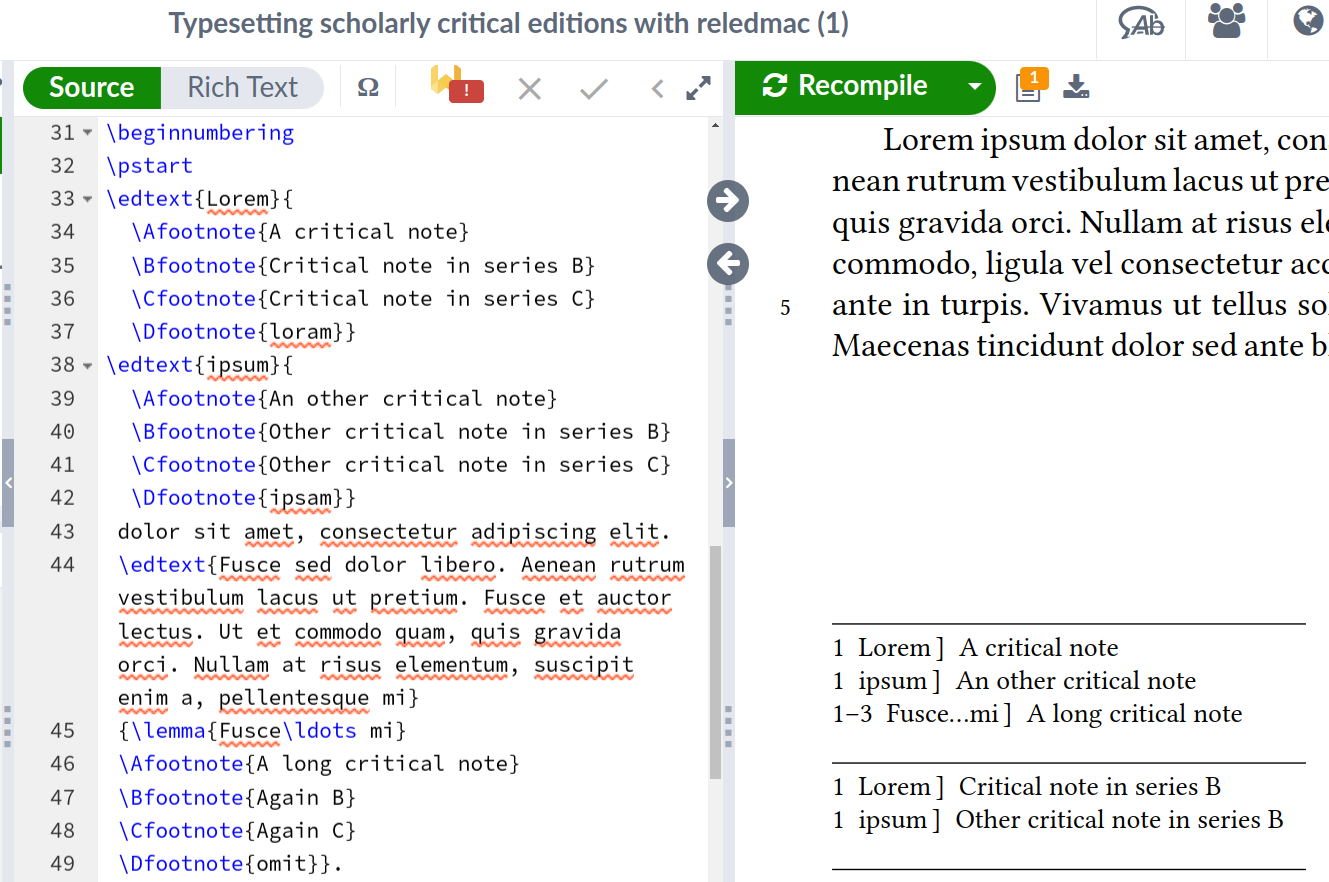
\includegraphics[width=0.8\textwidth]{img/overleaf-reledmac.png}
    
    \framebreak
    
    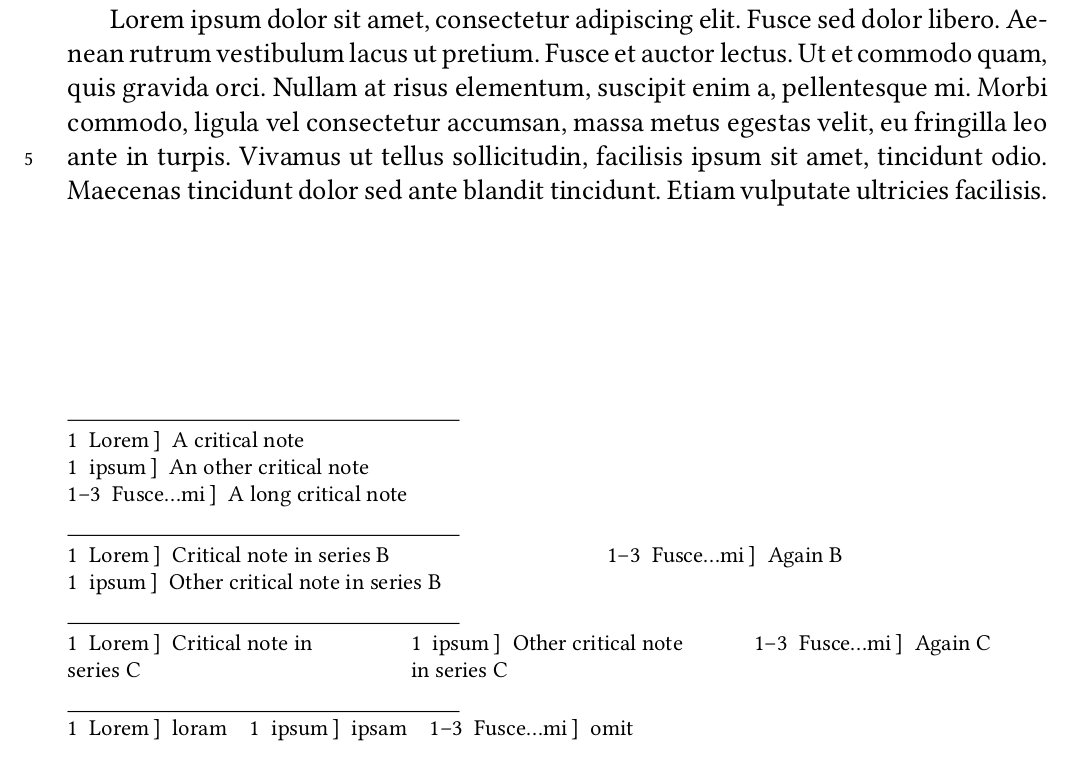
\includegraphics[width=0.8\textwidth]{img/overleaf-reledmac-pdf.png}
    
    \framebreak
    

    \begin{texcode}
\documentclass{article}
\usepackage{polyglossia,fontspec,xunicode}
\usepackage{libertine}
\setmainlanguage{latin}
\setotherlanguage{english}

\usepackage[series={A,B,C,D},noend,noeledsec,
            nofamiliar,noledgroup]{reledmac}
\Xarrangement[B]{twocol}
\Xarrangement[C]{threecol}
\Xarrangement[D]{paragraph}
\begin{document}

\title{Critical notes}
\maketitle

\beginnumbering
\pstart
\edtext{Lorem}{
  \Afootnote{A critical note}
  \Bfootnote{Critical note in series B}
  \Cfootnote{Critical note in series C}
  \Dfootnote{loram}}
\edtext{ipsum}{
  \Afootnote{An other critical note}
  \Bfootnote{Other critical note in series B}
  \Cfootnote{Other critical note in series C}
  \Dfootnote{ipsam}}
 dolor sit amet, consectetur adipiscing elit. 
 \edtext{Fusce sed dolor libero. Aenean rutrum vestibulum 
 lacus ut pretium. Fusce et auctor lectus. Ut et commodo 
 quam, quis gravida orci. Nullam at risus elementum, 
 suscipit enim a, pellentesque mi}
 {\lemma{Fusce\ldots mi}
 \Afootnote{A long critical note}
 \Bfootnote{Again B}
 \Cfootnote{Again C}
 \Dfootnote{omit}}. 
Morbi commodo, ligula vel consectetur accumsan, massa metus 
egestas velit, eu fringilla leo ante in turpis. Vivamus ut 
tellus sollicitudin, facilisis ipsum sit amet, tincidunt odio. 
Maecenas tincidunt dolor sed ante blandit tincidunt. 
Etiam vulputate ultricies facilisis.
\pend
\endnumbering
\end{document}
\end{texcode}
\end{frame}

%----------------------------------------------------
\begin{frame}[fragile, allowframebreaks]{Explantation of the \texttt{reledmac} example}
\metroset{block=fill}
\small

    The following loads the \texttt{reledmac} package with the option to have four different sets of critical notes.
    \begin{texcode}
\usepackage[series={A,B,C,D},noend,noeledsec,
            nofamiliar,noledgroup]{reledmac}
\Xarrangement[B]{twocol}
\Xarrangement[C]{threecol}
\Xarrangement[D]{paragraph}
    \end{texcode}
    
    \begin{block}{Explanation}
    This defines the following arrangement:
    \begin{description}\scriptsize
    \item[Each note of type A] gets its own paragraph.
    \item[Each note of type B] gets its own paragraph but notes arranged in \alert{2 columns}.
    \item[Each note of type C] gets its own paragraph but notes arranged in \alert{3 columns}.
    \item[Each note of type D] is in the same paragraph.
    \end{description}
    \end{block}
    
    \framebreak
    
    This is one note -- `lorem' in the \verb|\edtext|-command is the lemma on which the notes `hang', i.e. we open a nested list. With \verb|\Afootnote| we specify that the note should be added to the A apparatus (and so forth).
    \begin{texcode}
    \edtext{Lorem}{
  \Afootnote{A critical note}
  \Bfootnote{Critical note in series B}
  \Cfootnote{Critical note in series C}
  \Dfootnote{loram}}
    \end{texcode}
    
    The superstructure of all this is 
    \begin{texcode}
    \beginnumbering
    \pstart
    [one paragraph of edition stuff]
    \pend
    \endnumbering
    \end{texcode}
    
    \framebreak
    
    Special usecases, like a note spanning multiple lines, goes like this:
    \begin{texcode}
    \edtext{Fusce sed dolor libero. Aenean rutrum vestibulum lacus ut 
    pretium. Fusce et auctor lectus. Ut et commodo quam, quis gravida 
    orci. Nullam at risus elementum, suscipit enim a, pellentesque mi}
    {\lemma{Fusce\ldots mi}
    \Afootnote{A long critical note}
    [...]
    }
    \end{texcode}
    With \verb|\lemma| we define what the abbreviated lemma should look like in the apparatus. 
    
    The overleaf example also contains three more documents you might want to look at: \texttt{sidenotes.tex}, \texttt{tabular.tex} and \texttt{verses.tex}. 
    To get the result of their code, click into the document and then click `Recompile' from there. 
    
    \framebreak
    
    \begin{block}{Further reading}
    \begin{itemize}\footnotesize
        \item \textbf{A review on the RIDE journal:} {\scriptsize \emph{Reledmac. Typesetting technology-independent critical editions with LaTeX} = Reledmac, Maïeul Rouquette (ed.), 1987--2019. \protect\url{https://ctan.org/pkg/reledmac} (Last Accessed: 21.07.2019). Reviewed by Andrew N. J. Dunning. In \emph{RIDE – A review journal for digital editions and resources} 11 (Tools and Environments), 2020. \protect\url{https://ride.i-d-e.de/issues/issue-11/reledmac/}. }
        \item \textbf{Package documentation:} For more info, see the \href{https://ctan.org/pkg/reledmac}{\texttt{reledmac} package documentation} (496 pages). {\scriptsize You can make indices, glossaries -- all sorts of options are documented here. Also: read up on the history of the package. }
        %\item Examples on \texttt{reledmac}'s referencing system: see RIDE review (above).
        \item \textbf{\href{https://web.archive.org/web/20191211173459/http://teicat.huma-num.fr/}{Marjorie Burghart’s TEI Critical Apparatus Toolbox}} contains a tool to turn TEI into \texttt{reledmac} PDF edition. $\to$ \href{https://github.com/MarjorieBurghart/TEI-CAT/blob/master/tei2latex_final.xslt}{XSLT is here.}
        \begin{itemize}\scriptsize
            \item The web service gives you a \texttt{.zip} with the \texttt{.tex} code and the PDF generated from it. Or you can just transform it yourself, using the \href{https://github.com/MarjorieBurghart/TEI-CAT/blob/master/tei2latex_final.xslt}{XSL from Github}.
            \item Our template (\texttt{mini-latex-reledmac.xsl}) is a simplified version of it -- but with your new XSLT skills, you can make it your own (take what you need, leave what you don't).
        \end{itemize}
    \end{itemize}
    \end{block}
    
    
\end{frame}


%------------------------------------------------------------------------------
\begin{frame}[standout]
    \alert{\LaTeX{} Practice!} \\
    \normalsize
    To understand the basics of \LaTeX{} better, open the \alert{\href{https://www.overleaf.com/latex/templates/a-humanities-seminar-paper-with-latex-in-10min/zdnfrdtfcsdz}{Humanities' seminar paper with LaTeX in 10min} Overleaf template}. Read the code, comments and understand the resulting PDF.
    
    Open the \alert{\href{https://www.overleaf.com/latex/examples/typesetting-scholarly-critical-editions-with-reledmac/vwfgrsxqncvv}{\texttt{reledmac} template on Overleaf}} and play around with it. 
    
    Start working on the XPath/XSLT exercise sheet (resources/materials folder), XSLT 2.1 part and answer the same questions for \LaTeX{} (for example, taking the above \texttt{reledmac} template into account). Feel free to use the slides and cheatsheet for help.
    
\end{frame}





